\documentclass[12pt]{article}
\input{preamble}

\pagestyle{fancy}
\fancyhf{}

\rhead{Nørre Gymnasium\\
1.v
}
\cfoot{Side \thepage \hspace{1pt} af \pageref{LastPage}}

%Husk at rette modul og dato!
\lhead{Matematik B\\
Lineær vækst og lineære funktioner
}
\chead{ %25/3/2022
}

\begin{document}

%Udfyld afsnit herunder og lav til egen Latex-fil

%Kopier følgende til overskrift:

%\begin{center}
%\Huge
%Aflevering 1
%\end{center}
%\section*{Opgave 1}
%\stepcounter{section}
\begin{center}
\Huge
Lineær vækst og lineære funktioner
\end{center}
\stepcounter{section}
For to tal $a$ og $b$ kaldes en sammenhæng mellem en uafhængig variabel $x$ og en afhængig variabel $y$ på formen $y = ax + b$ for en lineær sammenhæng. Dette leder os til definitionen af en lineær funktion
\begin{defn}
En lineær funktion $f$ defineres som en funktion med forskrift
\begin{align*}
f(x) = ax + b,
\end{align*}
hvor $a$ og $b$ er vilkårlige reelle tal. 
\end{defn}

\begin{exa}
Vi har en lineær sammenhæng $y = 3x-4$. Her er $a = 3$ og $b = -4$. 
\end{exa}
\begin{exa}
Funktionen $f$ givet ved
\begin{align*}
f(x) = -10x+7
\end{align*}
er en lineær funktion med $a= -10$ og $b = 7$.
\end{exa}

Af Fig. \ref{fig:lingrow} og Fig. \ref{fig:lingrow2} kan det ses, hvordan lineær vækst udvikler sig.
\begin{figure}[H]
\center
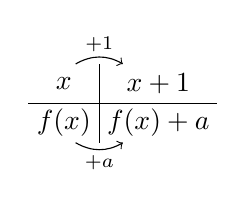
\begin{tikzpicture}
\foreach \i in {0}{
\draw (\i*0.9,0) -- (\i*0.9,1);
}
\draw (-0.9,0.5) -- (1.5,0.5);
\foreach \i in {0}{
\node at (\i*0.9+ 0.75,0.75) {$x+1$};
\node at (\i*0.9+0.75,0.25) {$f(x)+a$};
}
\node at (-0.45,0.75) {$x$};
\node at (-0.45,0.25) {$f(x)$};
\foreach \i in {0}{
\draw [->] (\i*0.9-0.3,1) to [out=30,in=150] (\i*0.9+0.3,1);
\node at (\i*0.9,1.25) {$\scriptstyle+1$};
\draw [->] (\i*0.9-0.3,-0) to [out=-30,in=-150] (\i*0.9+0.3,-0);
\node at (\i*0.9,-0.25) {$\scriptstyle + a$};
}
\end{tikzpicture}
\caption{Udvikling af lineær vækst.}
\label{fig:lingrow}
\end{figure}
\begin{figure}[H]
\centering
\begin{tikzpicture}
\begin{axis}[axis lines = middle, xtick = {3,5}, ytick = {1,3}, xmin = -3, xmax = 7, ymin = -3, ymax = 6,
xticklabels = {$x$,$x+1$},
yticklabels = {$f(x)$ , $f(x)+a$},
 legend pos = south east
]
\addplot[samples = 100, color = blue!40, domain = -3:7, thick] {x-2};
\draw [decorate,
    decoration = {calligraphic brace, mirror}] (axis cs:3,1) --  (axis cs: 5,1);
\draw [decorate,
    decoration = {calligraphic brace, mirror}] (axis cs:5.0,1) --  (axis cs: 5.0,3);
\node at (axis cs:4,0.5) {$\scriptsize 1$};
\node at (axis cs:5.5,2) {$\scriptsize a$}; 
\draw[dashed, color = gray] (axis cs:0,1) -- (axis cs:3,1);
\draw[dashed, color = gray] (axis cs:3,0) -- (axis cs:3,1);
\draw[dashed, color = gray] (axis cs:5,1) -- (axis cs:5,0);
\draw[dashed, color = gray] (axis cs:0,3) -- (axis cs:5,3);
\legend{f(x) = ax+b},
\end{axis}
\end{tikzpicture}
\caption{Udvikling af lineær vækst}
\label{fig:lingrow2}
\end{figure}

 Det er ikke svært at overbevise sig selv, om at dette er tilfældet. Øges $x$ med $1$ får vi
\begin{align*}
f(x+1) = a(x+1) +b = ax+b + a = f(x)+ a,
\end{align*}
hvoraf det ses, at en øgning af $x$ med $1$ tilsvarer en øgning af $f(x)$ med $a$. 

Det er muligt at bestemme en entydig lineær funktion, der skærer gennem to punkter $(x_1,y_1)$ og $(x_2,y_2)$. Formlen til at bestemme denne lineære funktion kalder vi for topunktsformlen for lineære funktioner. Den er givet af følgende sætning. 
\begin{setn}[Topunktsformlen for lineære funktioner]
Har vi to punkter $(x_1,y_1)$ og $(x_2,y_2)$, så kan vi finde en entydig lineær funktion $f$ givet ved
\begin{align*}
f(x) = ax+b,
\end{align*}
hvis graf skærer gennem disse punkter. Koefficienterne $a$ og $b$ er givet ved henholdsvist
\begin{align*}
a = \frac{y_2-y_1}{x_2-x_1}
\end{align*}
og 
$$b = y_1-ax_1 = y_2-ax_2.$$
\end{setn}
\begin{proof}
Vi antager, at en lineær funktion $f$ givet ved
\begin{align*}
f(x) = ax+b
\end{align*}
skærer gennem punkterne $(x_1,y_1)$ og $(x_2,y_2)$. Der må da gælde, at 
\begin{align*}
y_1 = ax_1 + b
\end{align*}
og 
\begin{align*}
y_2 = ax_2 + b.
\end{align*}
Vi trækker nu disse udtryk fra hinanden.
\begin{align*}
y_2 - y_1 &= \underbrace{ax_2+b}_{=y_2}-\underbrace{(ax_1+b)}_{=y_1}\\
&= ax_2 + b -ax_1 - b\\
&= a(x_2-x_1)
\end{align*}
Vi isolerer nu $a$ i dette udtryk og får
\begin{align*}
\frac{y_2-y_1}{x_2-x_1} = a
\end{align*}
Vi mangler nu kun at vise, hvordan vi bestemmer $b$. Vi ved, at $y_1 = ax_1 + b$. Isoleres $b$ i dette udtryk fås
\begin{align*}
b = y_1 - ax_1.
\end{align*}

\end{proof}
\end{document}

